\chapter{Examples}
\label{anexample}

\section{Fractals}
\label{fractals}
The \GrG\ package ships with samples for fractal generation. We will construct the Sierpinski triangle and the Koch snowflake. First of all we have to compile the model and rule set files. So execute in \GrG's \texttt{bin} directory
\begin{verbatim}
GrGen.exe ..\specs\sierpinski.grg
GrGen.exe ..\specs\snowflake.grg
\end{verbatim}
or
\begin{verbatim}
mono GrGen.exe ../specs/sierpinski.grg
mono GrGen.exe ../specs/snowflake.grg
\end{verbatim}
respectively. If you are on a Unix-like system you have to adjust the path separators of the \GrShell\ scripts. Just edit the first three lines of \texttt{/test/Sierpinski.grs} and \texttt{/test/Snowflake.grs}. And as we have the file \texttt{Sierpinski.grs} already opened, we can increase the number of iterations to get even more beautiful graphs. Just follow the comments. Be careful when increasing the number of iterations of Koch's snowflake -- \yComp's layout algorithm might need some time and attempts to layout it nicely.\\
\\
We execute the Sierpinski script by
\begin{verbatim}
grShell.exe ..\test\Sierpinski.grs
\end{verbatim}
or
\begin{verbatim}
mono grShell.exe ../test/Sierpinski.grs
\end{verbatim}
respectively. Because both of the scripts are using the debug mode, we complete execution by typing \texttt{r}(un). See \ref{grsthings} for further information. The resulting graphs should look like figures \ref{figsierp} and \ref{figsnowflake}.
\begin{figure}[htbp]
  \centering
  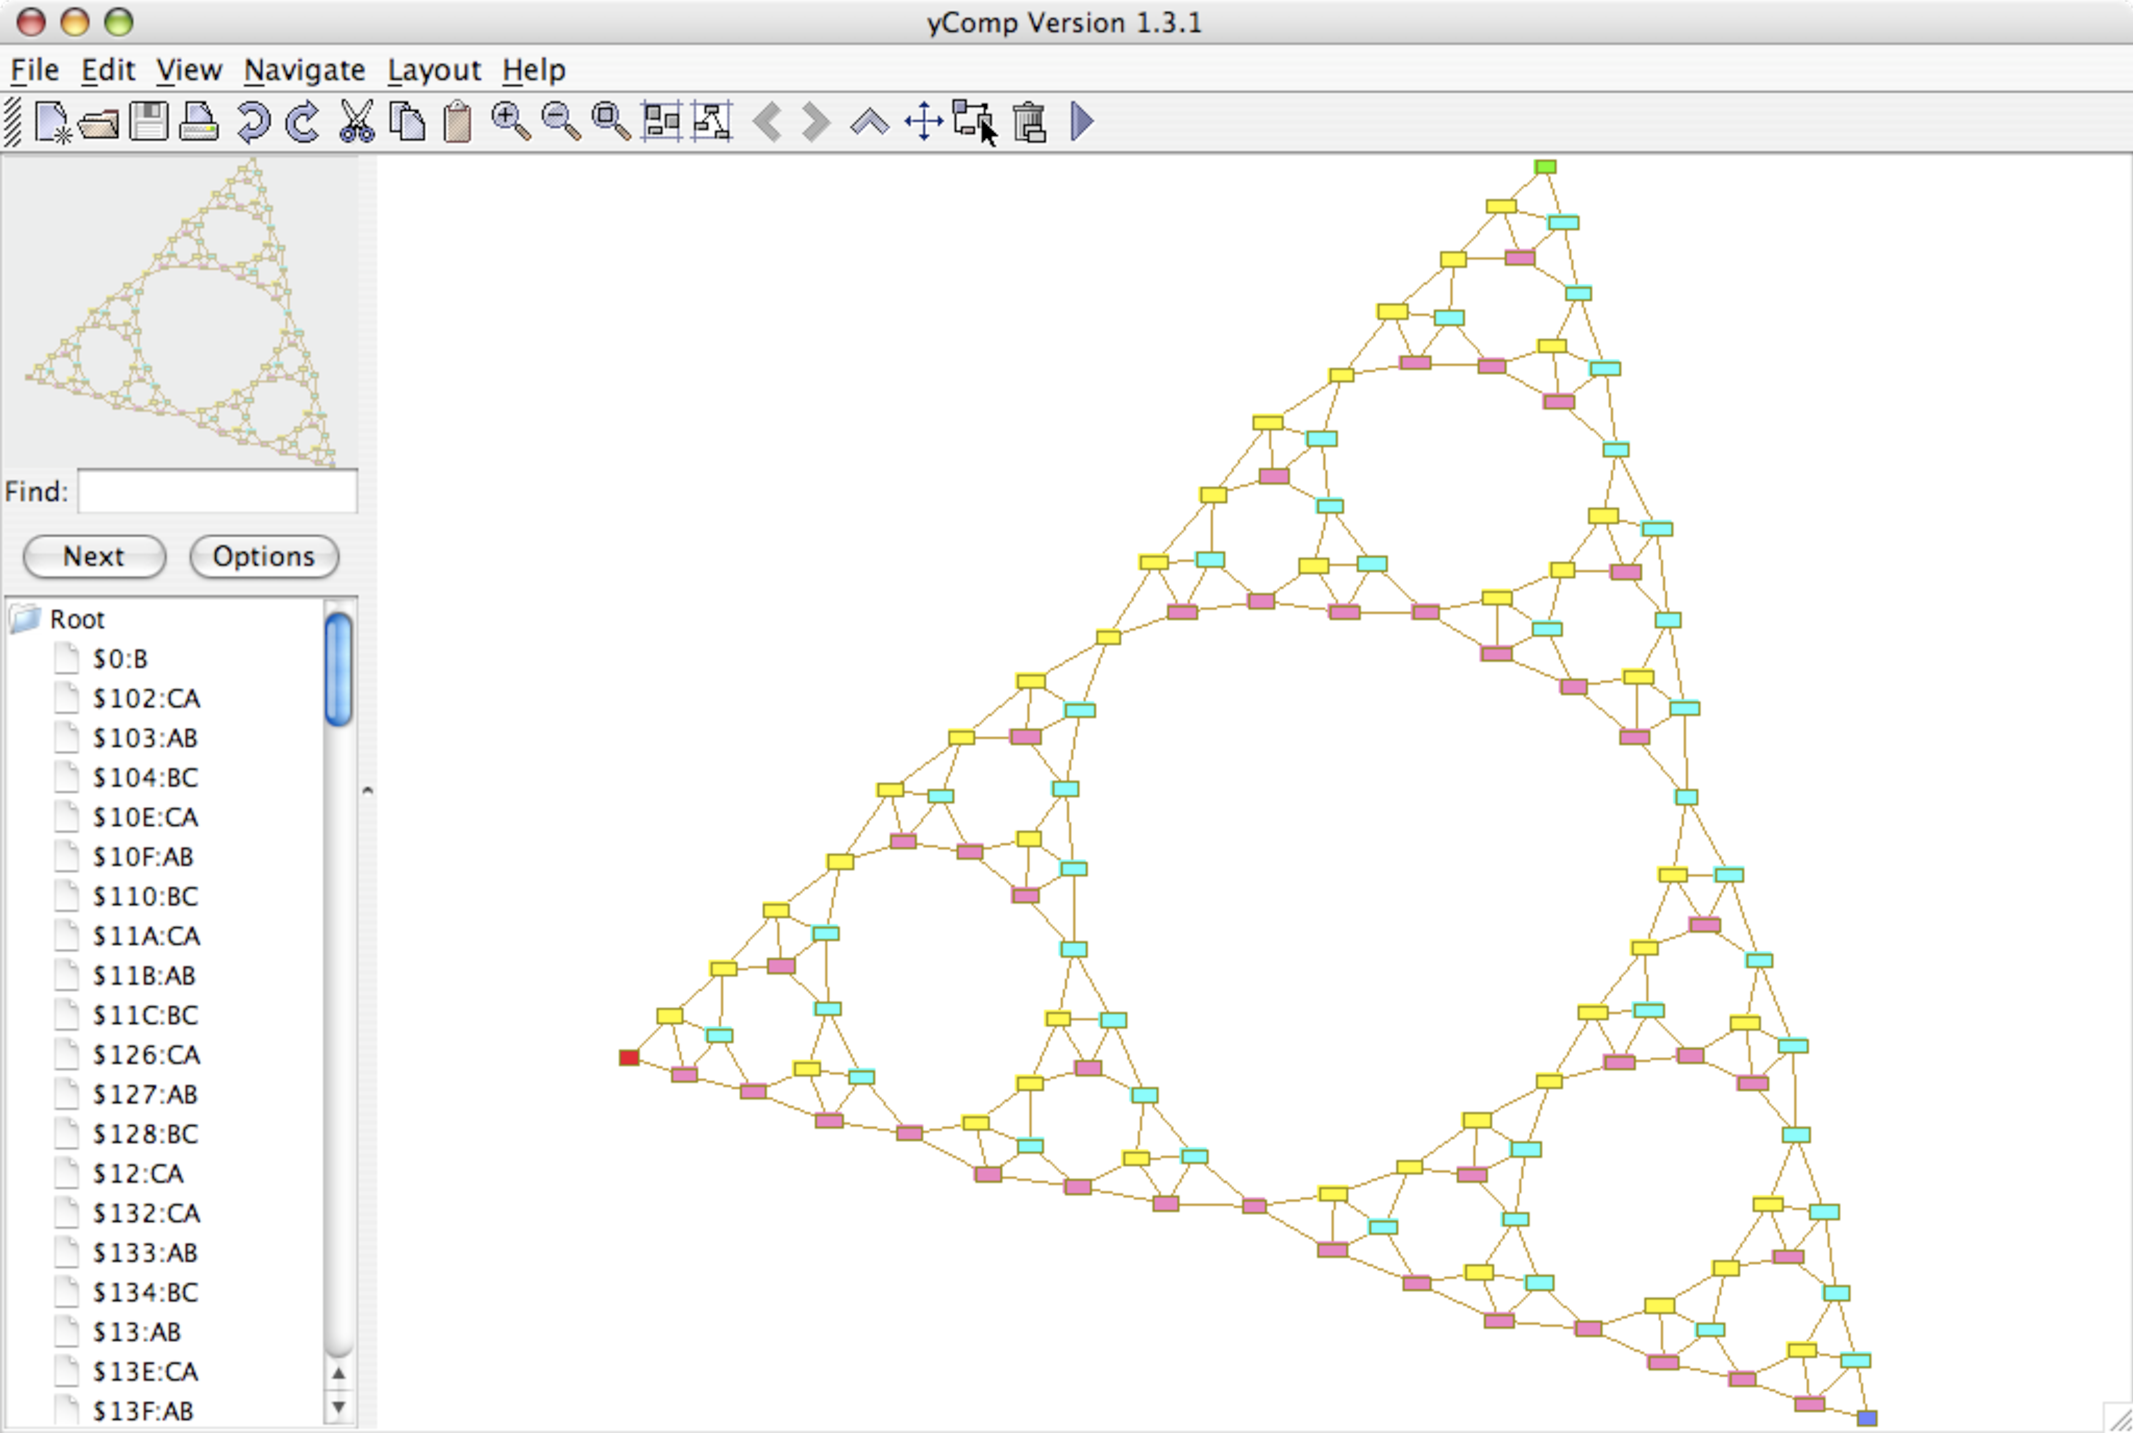
\includegraphics[width=\textwidth]{fig/sierpinski}
  \caption{Sierpinski triangle}
  \label{figsierp}
\end{figure}
\begin{figure}[htbp]
  \centering
  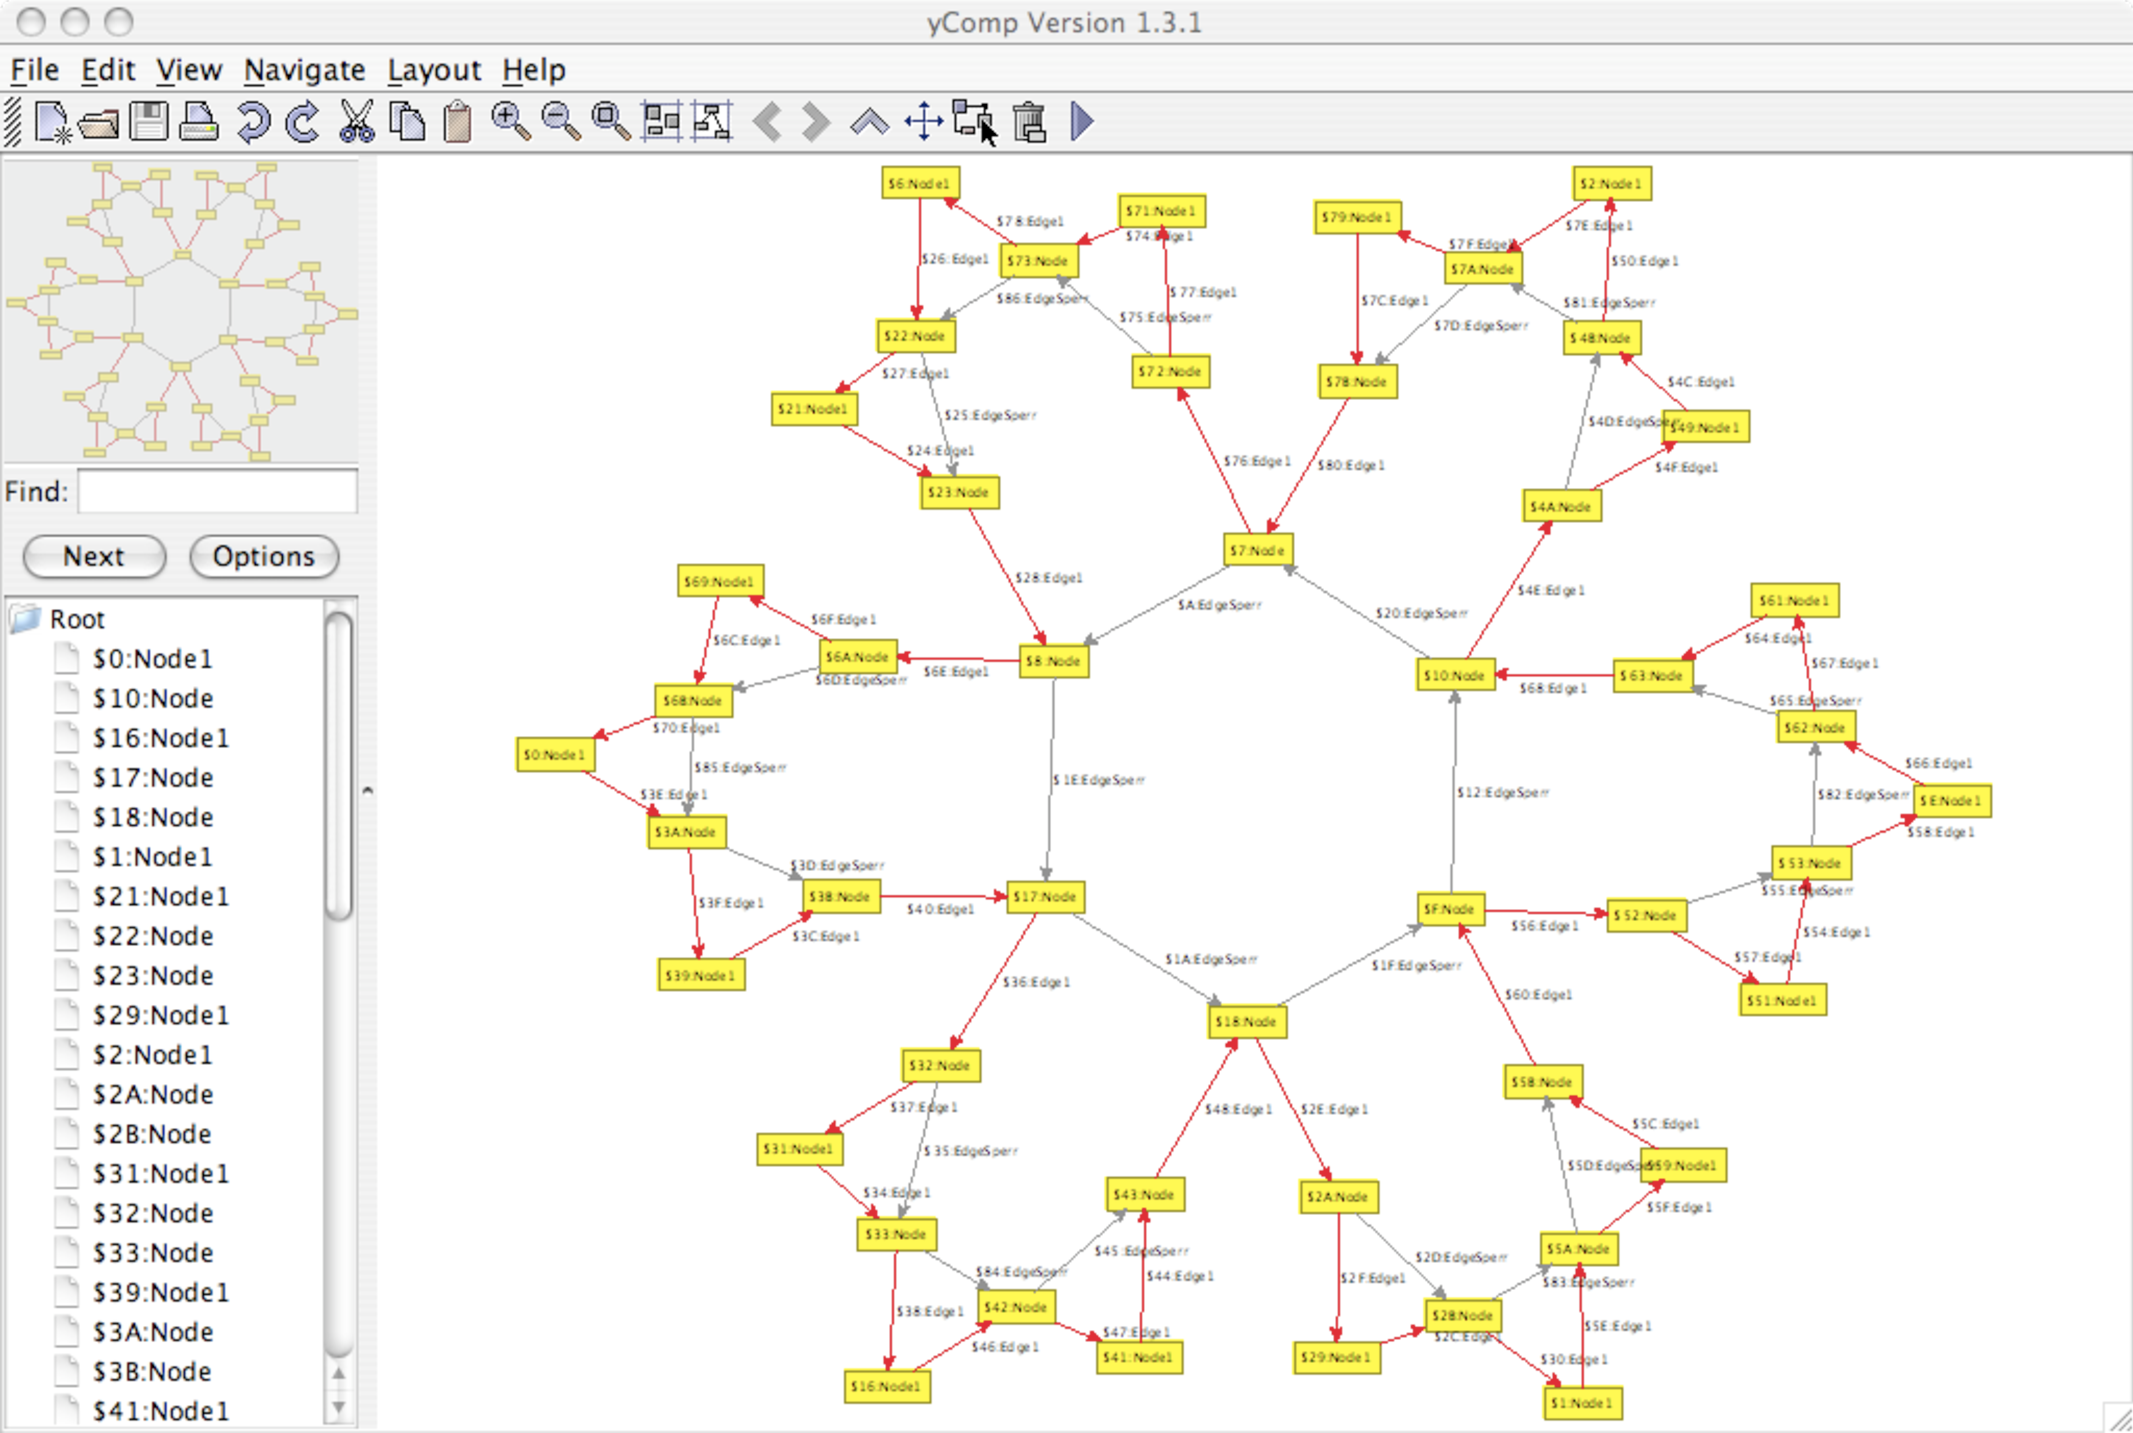
\includegraphics[width=\textwidth]{fig/snowflake}
  \caption{Koch snowflake}
  \label{figsnowflake}
\end{figure}


\section{Busy Beaver}
We want \GrG\ to work as hard as a busy beaver \cite{kroll, bb}. Our busy beaver is a Turing machine, that has got five states, writes 1,471 bars onto the tape and terminates \cite{beaver}. So first of all we design a Turing machine as graph model. Besides this example shows that \GrG\ is Turing complete. 

\subsection{Graph Model}
Let's start the model file \emph{TuringModel.gm} with
\begin{grgen}[firstnumber=1]
model TuringModel; 

\end{grgen}

The tape will be a chain of \emph{TapePosition} nodes connected by right edges. A cell value is modeled by a reflexive \emph{value} edge, attached to a \emph{TapePosition} node. The leftmost and the rightmost cell (\emph{TapePosition}) does not have an incoming and outgoing edge respectively. Therefore we have the node constraint $[0:1]$.
\begin{grgen}[firstnumber=last]
node class TapePosition; 
edge class right
  connect TapePosition[0:1] -> TapePosition[0:1];
  
edge class value
  connect TapePosition[1] -> TapePosition[1];  
edge class zero extends value;
edge class one extends value;
edge class empty extends value;

\end{grgen}
Finally we need states and transitions. The current configuration is modeled with a \emph{RWHead} edge pointing to a \emph{TapePosition} node. \emph{State} nodes are connected with \emph{WriteValue} nodes via \emph{value} edges and from a \emph{WriteValue} node a \emph{move\dots} edge leads to the next state.
\begin{grgen}[firstnumber=last]
node class RWHead;

node class WriteValue;
node class WriteZero extends WriteValue;
node class WriteOne extends WriteValue;
node class WriteEmpty extends WriteValue; 

edge class moveLeft;
edge class moveRight;
edge class dontMove;

\end{grgen}

\subsection{Rule Set}
Now the rule set: we begin the rule set file \emph{Turing.grg} with
\begin{grgen}[firstnumber=1] 
actions Turing using TuringModel;

\end{grgen}
We need rewrite rules for the following steps of the Turing machine:
\begin{enumerate}
  \item Read the value of the current tape cell and select an outgoing edge of the current state.
  \item Write a new value into the current cell, according to the sub type of the \emph{WriteValue} node.
  \item Move the read-write-head along the tape and propagate a new state as current state. 
\end{enumerate}
As you can see a transition of the Turing machine is split into two graph rewriting steps: Writing the new value onto the tape and performing the state transition. We need eleven rules, three rules for each step (for ``zero'', ``one'' and ``empty'') and two rules for extending the tape to the left and the right, respectively.
\begin{grgen}[firstnumber=last] 
rule readZeroRule {
	pattern {
		s:State -:RWHead-> tp:TapePosition -zv:zero-> tp;
		s -zr:zero-> wv:WriteValue;
	}
	replace {
		s -zr-> wv;
		tp -zv-> tp;
		wv -:RWHead->tp;
	}
}      

\end{grgen}
We take the current state \emph{s} and the current cell \emph{tp} implicitly given by the unique \emph{RWHead} edge and check, whether the cell value is zero. Furthermore we check if the state has a transition for zero. The replacement part deletes the \emph{RWHead} edge between \emph{s} and \emph{tp} and adds it between \emph{wv} and \emph{tp}. The remaining rules are analogous:
\begin{grgen}[firstnumber=last] 
rule readOneRule {
	pattern {
		s:State -:RWHead-> tp:TapePosition -ov:one-> tp;
		s -or:one-> wv:WriteValue;
	}
	replace {
		s -or-> wv;
		tp -ov-> tp;
		wv -:RWHead-> tp;
	}
}

rule readEmptyRule {
	pattern {
		s:State -:RWHead-> tp:TapePosition -ev:empty-> tp;
		s -er:empty-> wv:WriteValue;
	}
	replace {
		s -er-> wv;
		tp -ev-> tp;
		wv -:RWHead-> tp;
	}
}

rule writeZeroRule {
	pattern {
		wv:WriteZero -rw:RWHead-> tp:TapePosition -:value-> tp;
	}
	replace {
		wv -rw-> tp -:zero-> tp;
	}	
}

rule writeOneRule {
	pattern {
		wv:WriteOne -rw:RWHead-> tp:TapePosition -:value-> tp;
	}
	replace {
		wv -rw-> tp -:one-> tp;
	}	
}

rule writeEmptyRule {
	pattern {
		wv:WriteEmpty -rw:RWHead-> tp:TapePosition -:value-> tp;
	}
	replace {
		wv -rw-> tp -:empty-> tp;
	}	
}

rule moveLeftRule {
	pattern {
		wv:WriteValue -m:moveLeft-> s:State;
		wv -:RWHead-> tp:TapePosition <-r:right- ltp:TapePosition;
	}
	replace {
		wv -m-> s;
		s -:RWHead-> ltp -r-> tp;
	}
}

rule moveRightRule {
	pattern {
		wv:WriteValue -m:moveRight-> s:State;
		wv -:RWHead-> tp:TapePosition -r:right-> rtp:TapePosition;
	}
	replace {
		wv -m-> s;
		s -:RWHead-> rtp <-r- tp;
	}
}

rule dontMoveRule {
	pattern {
		wv:WriteValue -m:dontMove-> s:State;
		wv -:RWHead-> tp:TapePosition;
	}
	replace {
		tp;
		wv -m-> s;
		s -:RWHead-> tp;
	}
}

rule ensureMoveLeftValidRule {
	pattern {
		wv:WriteValue -m:moveLeft-> s:State;
		wv -rw:RWHead-> tp:TapePosition;
		negative {
			tp <-:right- ltp:TapePosition;
		}
	}
	replace {
		wv -m-> s;
		wv -rw-> tp <-:right- ltp:TapePosition -:empty-> ltp;
	}
}

rule ensureMoveRightValidRule {
	pattern {
		wv:WriteValue -m:moveRight-> s:State;
		wv -rw:RWHead-> tp:TapePosition;
		negative {
			tp -:right-> rtp:TapePosition;
		}
	}
	replace {
		wv -m-> s;
		wv -rw-> tp -:right-> rtp:TapePosition -:empty-> rtp;
	}
}
\end{grgen}
Have a look at the negative conditions within the \emph{ensureMove\dots} rules. They ensure, that the current cell is indeed at the end of the tape: an edge to a right / left neighbor cell must not exist. Now don't forget to compile your model and the rule set with \texttt{GrGen.exe} (see \ref{fractals}).

\subsection{Rule Execution with \GrShell}

Finally we construct the busy beaver and let it work with \GrShell:
\begin{grshell}[firstnumber=1] 
select backend "lgspBackend.dll"
new graph "../lib/lgsp-TuringModel.dll" "Busy Beaver"
select actions "../lib/lgsp-TuringActions.dll"

# Initialize tape
new tp:TapePosition($="Startposition")

# States
new sA:State($="A")
new sB:State($="B")
new sC:State($="C")
new sD:State($="D")
new sE:State($="E")
new sH:State($ = "Halt")

new sA -:RWHead-> tp

# Transitions: three lines per state for
#   - updating cell value
#   - moving read-write-head
# respectively

new sA_0: WriteOne
new sA -:empty-> sA_0
new sA_0 -:moveLeft-> sB

new sA_1: WriteOne
new sA -:one-> sA_1
new sA_1 -:moveLeft-> sD

new sB_0: WriteOne
new sB -:empty-> sB_0
new sB_0 -:moveRight-> sC

new sB_1: WriteEmpty
new sB -:one-> sB_1
new sB_1 -:moveRight-> sE

new sC_0: WriteEmpty
new sC -:empty-> sC_0
new sC_0 -:moveLeft-> sA

new sC_1: WriteEmpty
new sC -:one-> sC_1
new sC_1 -:moveRight-> sB

new sD_0: WriteOne
new sD -:empty-> sD_0
new sD_0 -:moveLeft->sE

new sD_1: WriteOne
new sD -:one-> sD_1
new sD_1 -:moveLeft-> sH

new sE_0: WriteOne
new sE -:empty-> sE_0
new sE_0 -:moveRight-> sC

new sE_1: WriteOne
new sE -:one-> sE_1
new sE_1 -:moveLeft-> sC
}

\end{grshell}

Our busy beaver looks like this:
\begin{center}
  \fbox{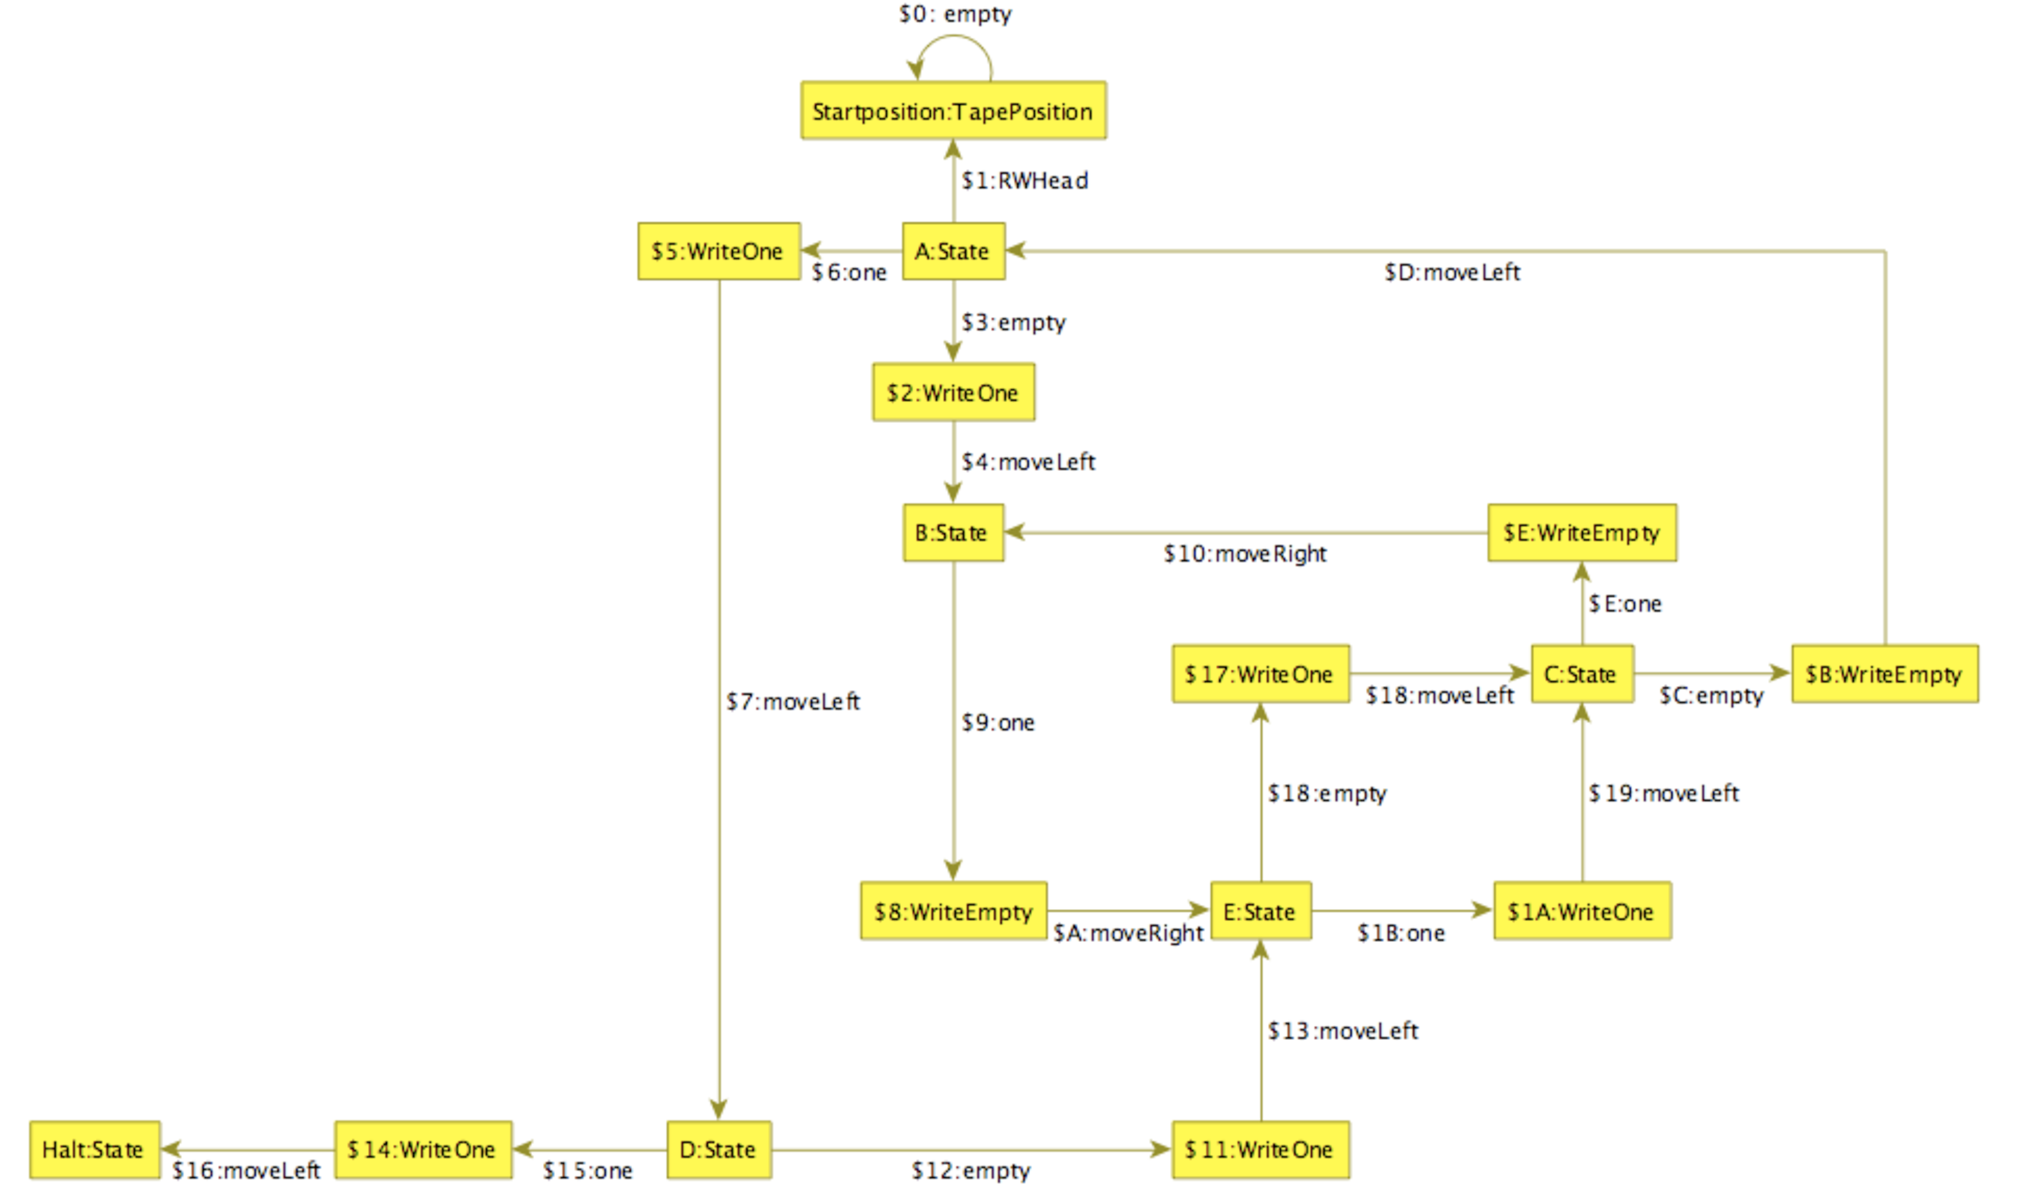
\includegraphics[width=\linewidth]{fig/bbstart}}
\end{center}
The graph rewriting sequence is quite straight forward and generic to the Turing graph model. Note that for each state the ``\emph{\dots Empty\dots} | \emph{\dots One\dots}'' selection is unambiguous.
\begin{grshell}[firstnumber=last]
  grs ((readOneRule | readEmptyRule) ; (writeOneRule | writeEmptyRule) ; (ensureMoveLeftValidRule | ensureMoveRightValidRule) ; (moveLeftRule | moveRightRule)){32}

\end{grshell}
We intercept the machine after 32 iterations and look at the result so far:
\begin{center}
  \fbox{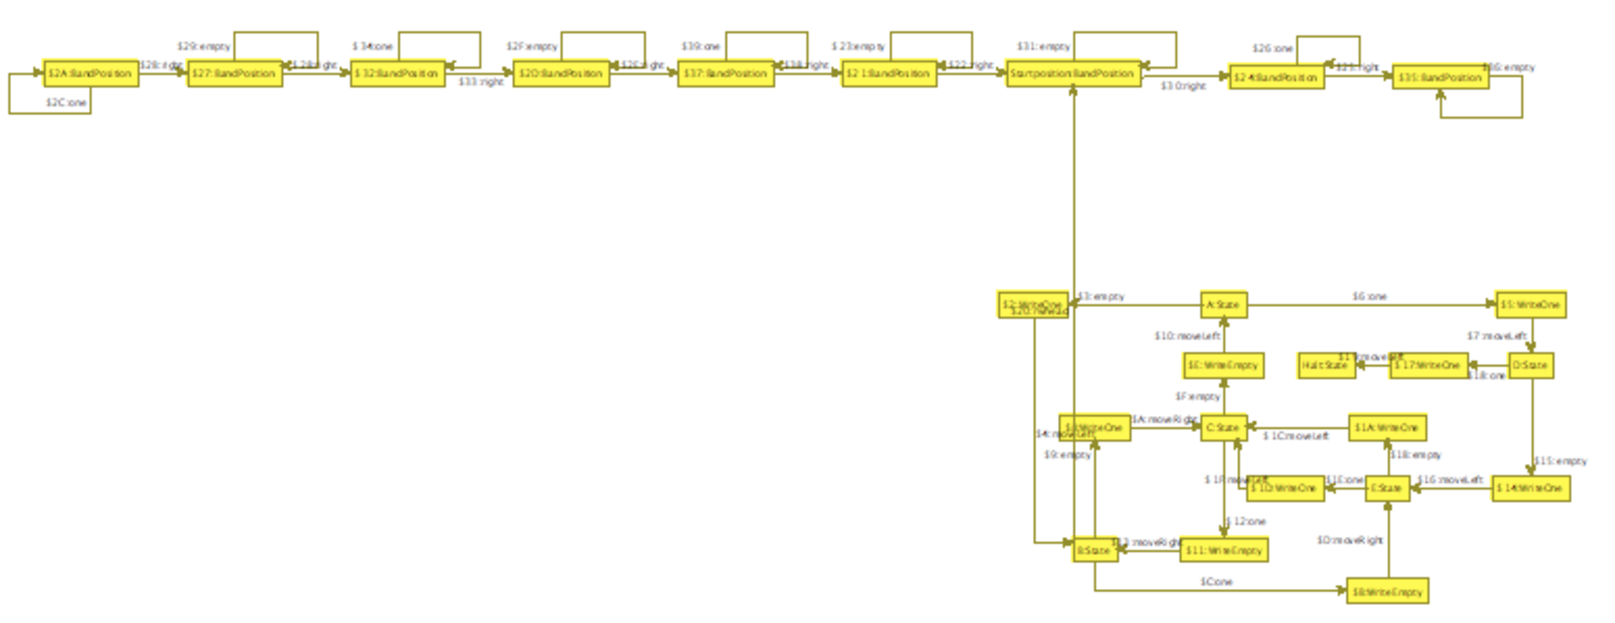
\includegraphics[width=\linewidth]{fig/bbmiddle}}
\end{center}
In order to improve the performance we generate better search plans. This is a crucial step for execution time: with the initial search plans the beaver runs for 9 minutes. With improved search plans after the first 32 steps he takes about 170 seconds.
\begin{grshell}[firstnumber=last]
custom graph analyze_graph
custom actions gen_searchplan readOneRule readEmptyRule writeOneRule writeEmptyRule ensureMoveLeftValidRule ensureMoveRightValidRule moveLeftRule moveRightRule

\end{grshell}

Let the beaver run:
\begin{grshell}[firstnumber=last]
  grs ((readOneRule | readEmptyRule) ; (writeOneRule | writeEmptyRule) ; (ensureMoveLeftValidRule | ensureMoveRightValidRule) ; (moveLeftRule | moveRightRule))*

\end{grshell}

